No es un secreto de que llevar a cabo una misión satelital representa grandes costos
y largos periódos de tiempo de desarrollo de la misión.
La NASA también padeció estos problemas hace algunas décadas.
Pero aquella, al ser una organización consciente de sus habilidades (y sobre todo con recursos),
se puede dar el lujo de innovar, de ir en contra de las corriente y filosofías normales de desarrollo.
Así, es como surge su lema \textit{Faster, Better and Cheaper} (FBC).
Este lema fue introducido por el administrador de la NASA Dan Goldin a
principios de la decáda de los 90's. Dan Goldin tiene una basta experiencia en
el desarrollo de pequeños satélites. Él estaba convencido de que el desarrollo
``clásico'' de misiones satelitales de NASA necesitaba un cambio de enfoque,
para lograr reducir el tiempo de desarrollo, y pasar de escalas de tiempo de
décadas a años y sobre todo lograr reducir costos \citep{Paxton07}.

Es sabido que este lema produce una gran cantidad de fallas y
carencias en las misiones satelitales \citep{Paxton07}. Sin embargo,
esto es lo que impulsa la innovación, y el desarrollo y entrenamiento de nuevos
managers, ingenieros y científicos, los cuales serán los líderes de las
nuevas generaciones. \citep{Paxton07}. Por tales motivos, es importante,
que empresas y organizaciones del ambito espacial en Argentina, dejen
de lado el ``clasicismo'', y se deben animar, y por su puesto, alentar a las futuras
generaciones, a transformar el tradicional \textit{caminar con los manuales de NASA bajo
  el brazo},  por la innovación y el desarrollo de nuevas tecnologías y técnicas
para la realización de satelites (que en este trabajo se denominan
\textit{vehículos de nueva generación}). Esta visión la tiene empresas tales como INVAP,
y otras tanto nacionales como extranjeras,  que están creciendo a paso agigantados llevando
en su interior el cambio de filosofía que se exige, para reducir costos, y con la capacidad
necesaria para producir a gran escala.

Este trabajo tiene como objetivo demostrar que es posible desarrollar
vehículos espaciales utilizando componentes COTS de baja confiabilidad, trayendo
consigo una reducción considerable del costo y del tiempo de desarrollo. De más está
decir, que esta tesis no busca desarrollar en profundidad una arquitectura
altamente confiable llegando a niveles de detalles,que son esperables en una misión satelital, en la
que participan varios equipos de decenas de ingenieros, managers y científicos. Si no,
más bien, ser el puntapié inicial de diversas líneas de investigación y desarrollo,
ya que como se ha demostrado en este trabajo, es factible el desarrollo de estas arquitecturas
``económicas'', con la aplicación de técnicas y filosofías que escapan de lo tradicional.

Luego de llevar a cabo un análisis de los sistemas satelitales y de aviónica que se
han publicado en diferentes trabajos de investigación, y como resultado de  diversas reuniones
con diferentes equipos dentro de la Unidad de Desarrollo INVAP, se llegó a la conclusión,
de que se debe trabajar sobre el  desarrollo de aviónicas confiables,
aún cuando sus componentes sean de baja confiabilidad, la comunicación entre componentes,
y que existe una tendencia a implementar redes de componentes dentro de los sistemas.

Así, una vez realizado este análisis previo, se estudiaron diferentes redes que tengan
la característica de ser tolerante a fallas y que sean factibles de ser
aplicadas en el ambiente espacial, estas se estudiaron en el Marco
Teórico (Capítulo \ref{chap:marco_teorico} Página \pageref{chap:marco_teorico}) y en
el Estado del Arte (Capítulo \ref{chap:estado_del_arte} Página \pageref{chap:estado_del_arte}).
Las cuales fueron las siguientes:
\begin{itemize}
\item Árboles binarios
\item Redes hypercube
\item Redes distribuídas
\end{itemize}

Los resultados del análisis de la confiabilidad se encuentra detallada en la sección
\ref{seccion:TopologiaEstudio} (Página \pageref{seccion:TopologiaEstudio}) y en
\cite{Arias17}. Resumiendo como se puede observar en la Figura
\ref{fig:comparative_reliablitiesConclusion}, la que presenta un mayor grado
de confiabilidad sostenible en el tiempo es la que corresponde a
la red distribuida. Este resultado representa un importante aporte para el
conocimiento de tipos de topologías confiables tolerantes a fallas, y el desarrollo de
modelos para lograr medir la confiabilidad de esas topologías. Los resultados de
este estudio fueron presentados en el \textit{Congreso Argentino de Tecnologías
  Espaciales 2017 (Córdoba, Argentina)}

\begin{figure}[H]
 \centering
 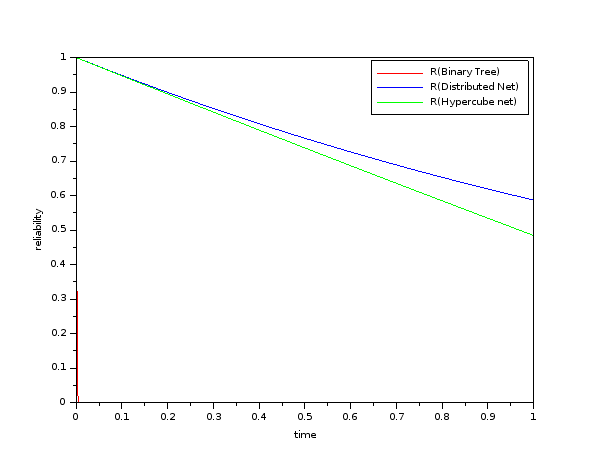
\includegraphics[scale=0.5]{images/Capitulo4/comparative_reliablities.png}
  \caption{Comparación de confiabilidad}
\label{fig:comparative_reliablitiesConclusion}
\end{figure}

Un requerimiento que fue planteado por la Unidad de Desarrollo INVAP fue trabajar
con el bus de comunicación CAN. CAN, es un protocolo de comunicación de bajo nivel,
que demuestra ser altamente confiable por lo que es utilizado (y es de donde nació)
mayormente en la industria automotriz. Esto, nos da una clara razón de que CAN, es un
protocolo confiable, debido a que en la fabricación de automóviles, el producto final
(el automóvil) puede poner en riesgo la vida de personas. Debido a su confiabilidad,
y a su excelente respuesta en sistemas de tiempo real, CAN es utilizado en también en
el ambiente espacial (entre otras industrias).

En base a estos resultados y restricciones se plantea el desafío de implementar,
crear, diseñar, una arquitectura que sea capaz de trabajar, con una filosofia
de red distribuida, esta puede estudiarse en \ref{chap:arquitectura_propuesta}
(Página \pageref{chap:arquitectura_propuesta}). El grado de innovación que coloca
esta nueva arquitectura se ve reflejada en que no existe una computadora única (la
connotación ``única'' hace referencia a la computadora propiamente dicha más sus
redundancias, o bien, cualquier (micro)controlador más sus redundancias) por cada
subsistema como se trabaja ``tradicionalmente'' sino que, existen computadoras
híbridas capaz de llevar a cabo tareas de todos los sistemas en forma distribuida. 

Para ello se planteó un protocolo basado en CAN y CANOpen. Este protocolo, hasta el
momento de desarrollar este trabajo, se encuentra en su versión 0.1 Alpha. El protocolo
presenta la innovación de estar orientado a objetos, y para ello se utilizó el
lenguaje SysML (System Modeling Language) para llevar a cabo su modelado y
la documentación del mismo. Estofacilita la interpretación del
stack de servicio que deben ser implementados a la hora del desarrollo. Este protocolo
se encuentra documentado en el apéndice \ref{Appendix:A} (Página \pageref{Appendix:A}).

En base a los resultados obtenidos y a la arquitectura propuesta basada en CANae
(apéndice \ref{Appendix:A}) se concluye de que es factible la desarrollar una
\textit{arquitectura de aviónica tolerantes a fallas basada en componentes COTS para
  vehículos satelitales} utilizando el bus CAN, como bus principal de comunicación.

\section{Cumplimiento de los objetivos}

\section{Trabajos a futuros}
Luego de desarrollado este trabajo de tesis, se logra ver el gran potencia que existe
en el estudio de arquitecturas de aviónicas tolerantes a fallas, y el estudio
de los componentes COTS introducidos en sistemas, donde el sistema esperado debe ser
más confiable que los componentes que la conforman.

Para ello se recomienda proseguir con los siguientes líneas de trabajo futuros:
\begin{itemize}
\item 
\end{itemize}

